\clearpage
\section{W tagging scale factor}
\subsection{Summary of differences with AN-13-139}
\begin{itemize}
\item
Matching: We match the subjets of a W-candidate to the daughters of the generator W, rather than matching the generator W to the W-candidate.
\item
dR cut: We include a dR cut between the W and b candidates.
\item
Inclusion of "loose" non-peaking Ws: Our efficiency takes into account any jet which is matched, regardless of whether or not they are in the W-peak.
\end{itemize}
\subsection{Selection}
We hope to use the hadronic $W$ from semileptonic $t\overline{t}$ decays as a representative sample. To isolate $W$-candidates, we apply the following selection:
\begin{enumerate}
\item
Require one muon with $p_T > 30$GeV.
\item
Require the muon be isolated. We use the cut: $\frac{\texttt{pfiso}^\mu}{p^\mu_T} > 0.12$.
\item
Require missing transverse momentum: $E^{miss}_T > 70$GeV 
\end{enumerate}
We then define a hemisphere around the muon, so that any object within $\Delta R < \pi/2$ of the muon is said to be in the \textit{leptonic} hemisphere. Any object not in this hemisphere is said to be in the \textit{hadronic} hemisphere. We then make the following cuts:
\begin{enumerate}
\item
We require the missing transverse energy to be in the same hemisphere as the muon.
\item
We require one jet with $p_T > 200$GeV in the leptonic hemisphere.
\item
We require on jet with $p_T > 200$GeV (this is the $W$-candidate) and one jet with $p_T > 30$GeV (the $b$-candidate) in the hadronic hemisphere.
\item
We require \textit{either} a b-tag on the $b$-candidate or on the leptonic hemisphere jet. Requiring two b-tags or only hadronic b-tags reduces our statistics so much that an effective measurement cannot be made.
\item
Finally, we require the total event mass from the sum of the muon and three jets to be greater than $300$GeV/c$^2$.
\end{enumerate}
\subsubsection{$\tau 2/\tau 1$ cut}
We sort the $W$-candidates into three distributions:
\begin{enumerate}
\item
TIGHT: $W$-candidates with $\tau 2/\tau 1 < 0.5$.
\item
LOOSE: $W$-candidates with $0.5 < \tau 2/\tau 1 < 0.75$. Note that the loose and tight cuts are exclusive.
\item
FAILED: $W$-candidates with $\tau 2/\tau 1 > 0.75$
\end{enumerate}
\subsubsection{Backgrounds}
These cuts are susceptible to three non-negligible backgrounds which contribute mostly to the loose and failed regions:
\begin{enumerate}
\item
Fully-leptonic $t\overline{t}$, with cross-section $25.17$pb.
\item
Single top from six different channels, with total cross-section of order $\sim40$pb.
\item
$W$+jets: this background is barely visible in MC (with our selection permitting only ~$10^{-5}\%$ events to pass the cuts). However, $W$+jets has a very high cross-section: $33836.9$pb, resulting in a non-negligible contribution.
\item
QCD: We found the QCD background to be negligible.
\end{enumerate}
The summed distributions of these backgrounds and the semi-leptonic $t\overline{t}$ for tight, loose, and failed are shown in figures \ref{fig:tightHIST}, \ref{fig:looseHIST} and, \ref{fig:failedHIST}.
\subsubsection*{Matched vs. Unmatched W-candidates}
The measurement of the scale factor should only consider true $W$s. In addition to separating the $W$-candidates from semi-leptonic $t\overline{t}$ and those from the various backgrounds, we must be able to discriminate between real $W$s in semi-leptonic $t\overline{t}$ and other jets which pass the selection. We match $W$-candidates by requiring that each of the jet's subjets lie within $\Delta R < 0.3$ of a $W$-daughter.
We are then left with five samples: matched semi-leptonic $t\overline{t}$, unmatched semi-leptonic $t\overline{t}$, all-leptonic $t\overline{t}$ background, $W$+jets background, and single top background. Each of these is split between tight, loose and failed shapes. 
 
\subsubsection{b-W Separation}
While investigating the relative separations of the various objects in an event, we noticed that some discrimination between matched and unmatched $W$s in semileptonic $t\overline{t}$ can be achieved through a cut on the $\Delta R$ of these jets ($\Delta R(Wjet, bjet)$). The two dimensional distribution of $\Delta R$ and $\tau 2/\tau 1$ for $W$ candidates is shown in Figure \ref{fig:drcut}. We make a cut on $\Delta R < 1.6$. Notice that the tight and loose peaks can be seen in the matched sample.
\begin{figure}[h!]
\centering
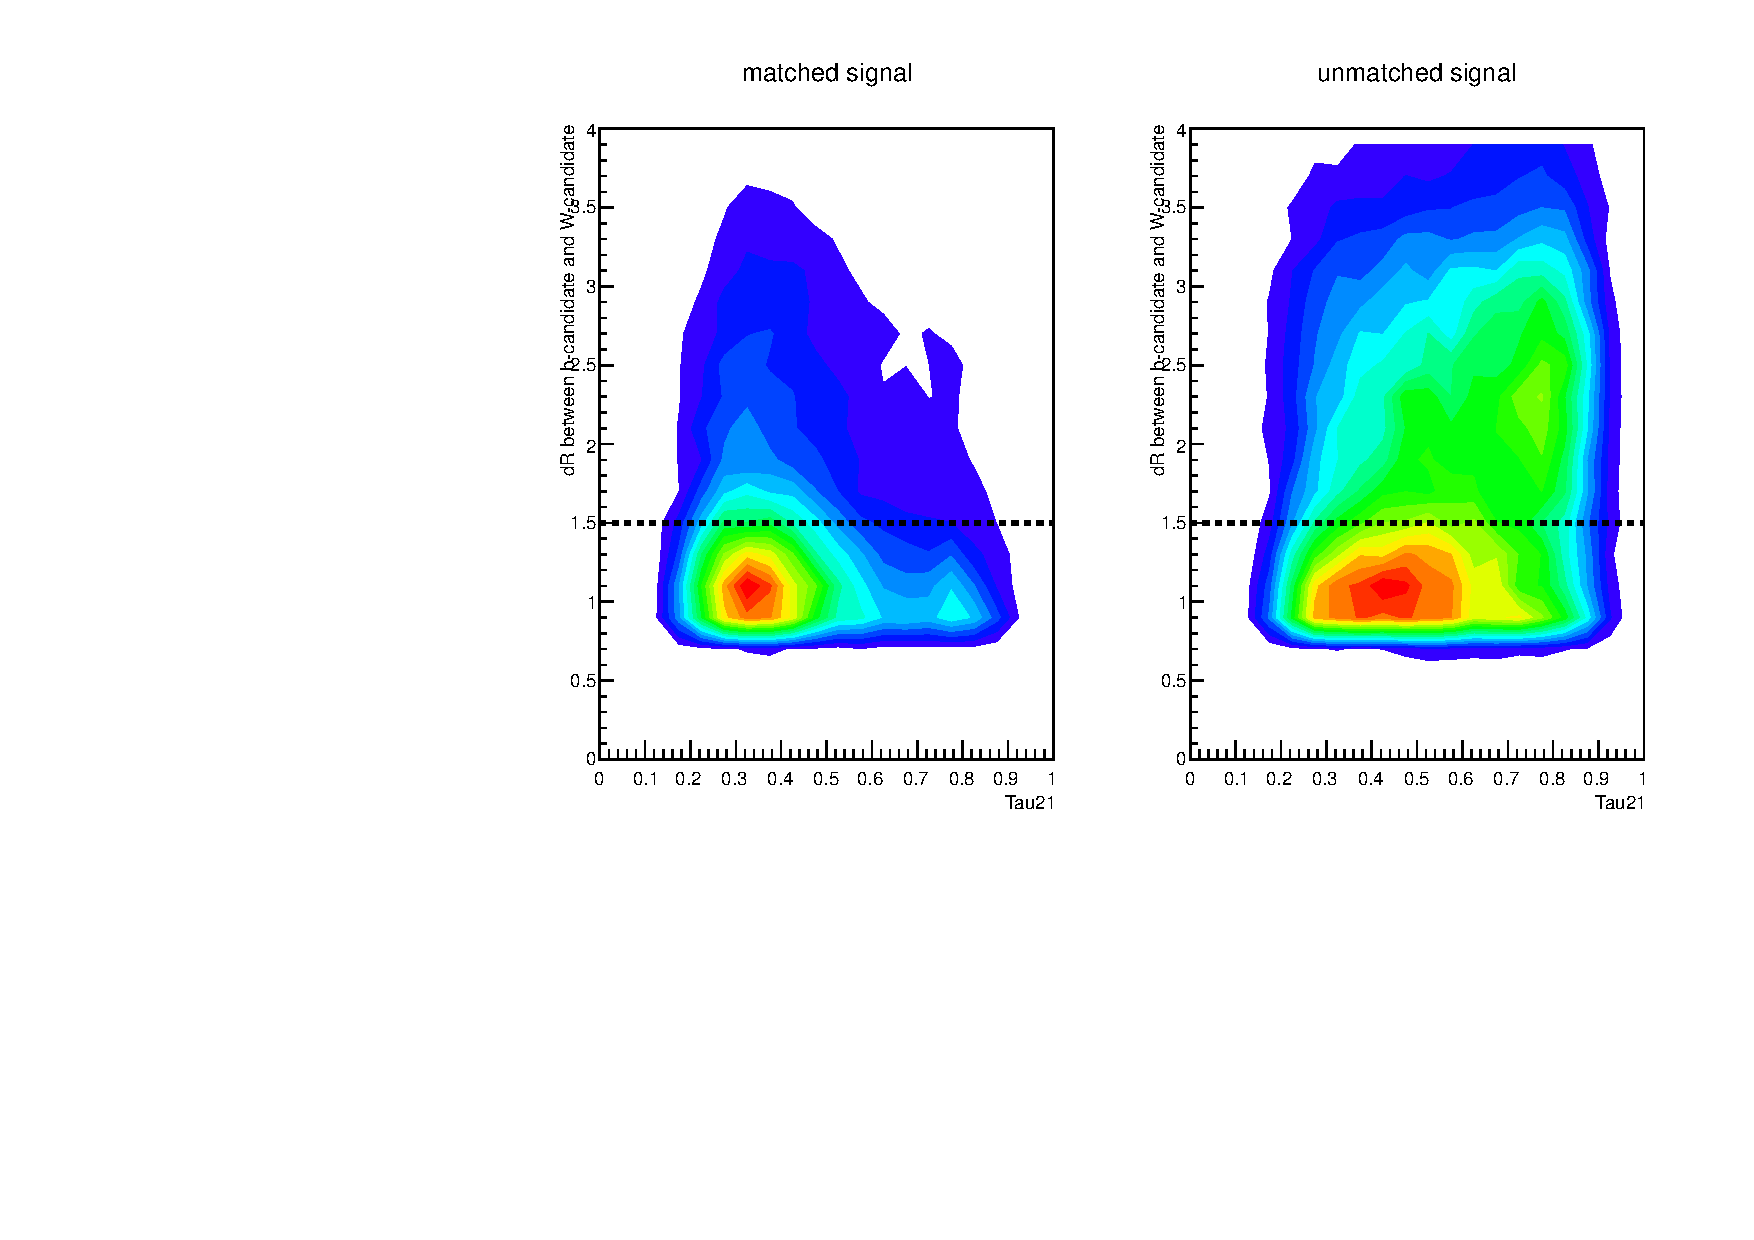
\includegraphics[scale=0.87]{EXO-12-024/figs/WtagSF/Z.pdf}
\caption{Distribution of $\Delta R$ and $\tau 2/\tau 1$ for $W$ candidates. The dotted black line shows the cut $\Delta R < 1.6$. The cut removes all events above the dotted line. Note that this cut is uncorrelated with $\tau 2/\tau 1$.}\label{fig:drcut}
\end{figure}
This cut does not change the shape of the $W$-mass distribution, only their normalizations. The effect of the cut can be seen in Figure~ \ref{fig:drproof}.
\begin{figure}[h!]
\centering
        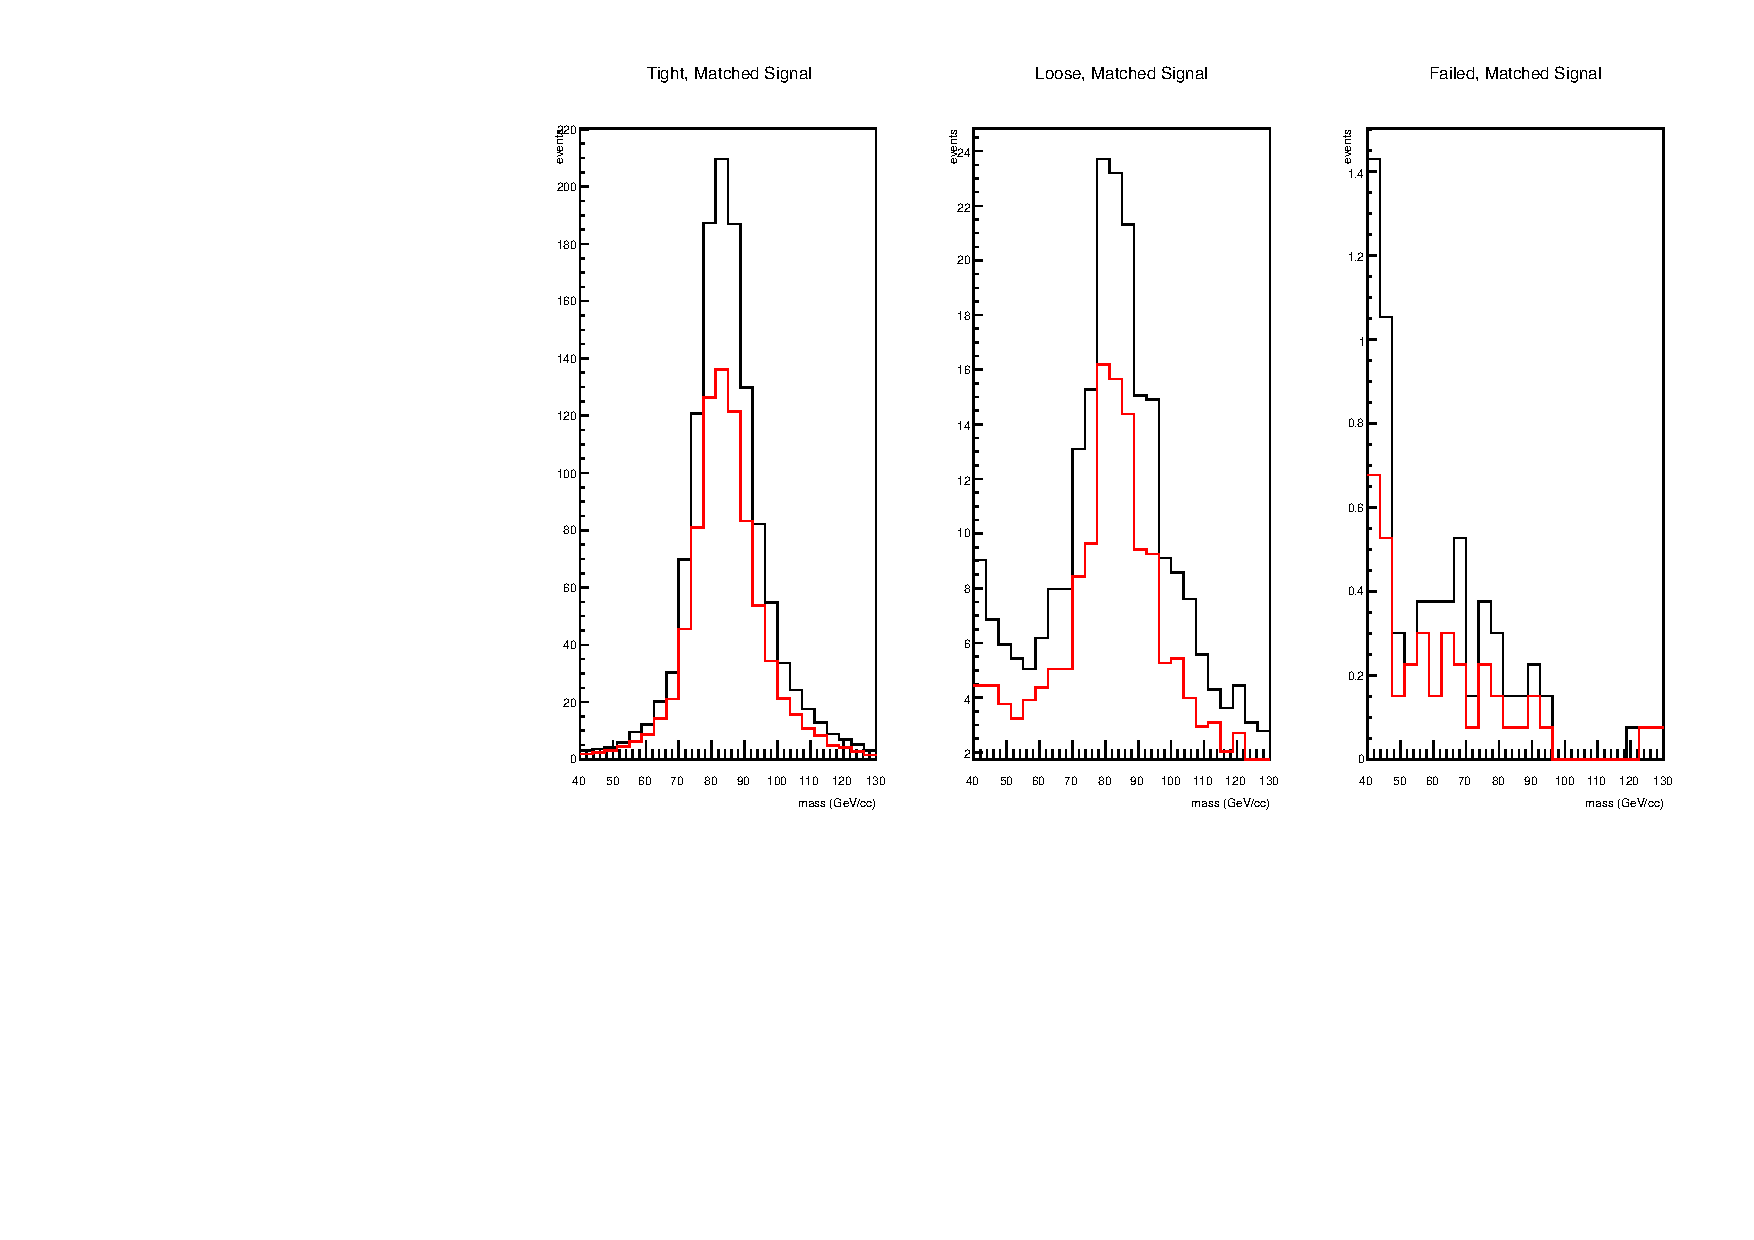
\includegraphics[width=0.77\textwidth]{EXO-12-024/figs/WtagSF/sigproof.pdf}
        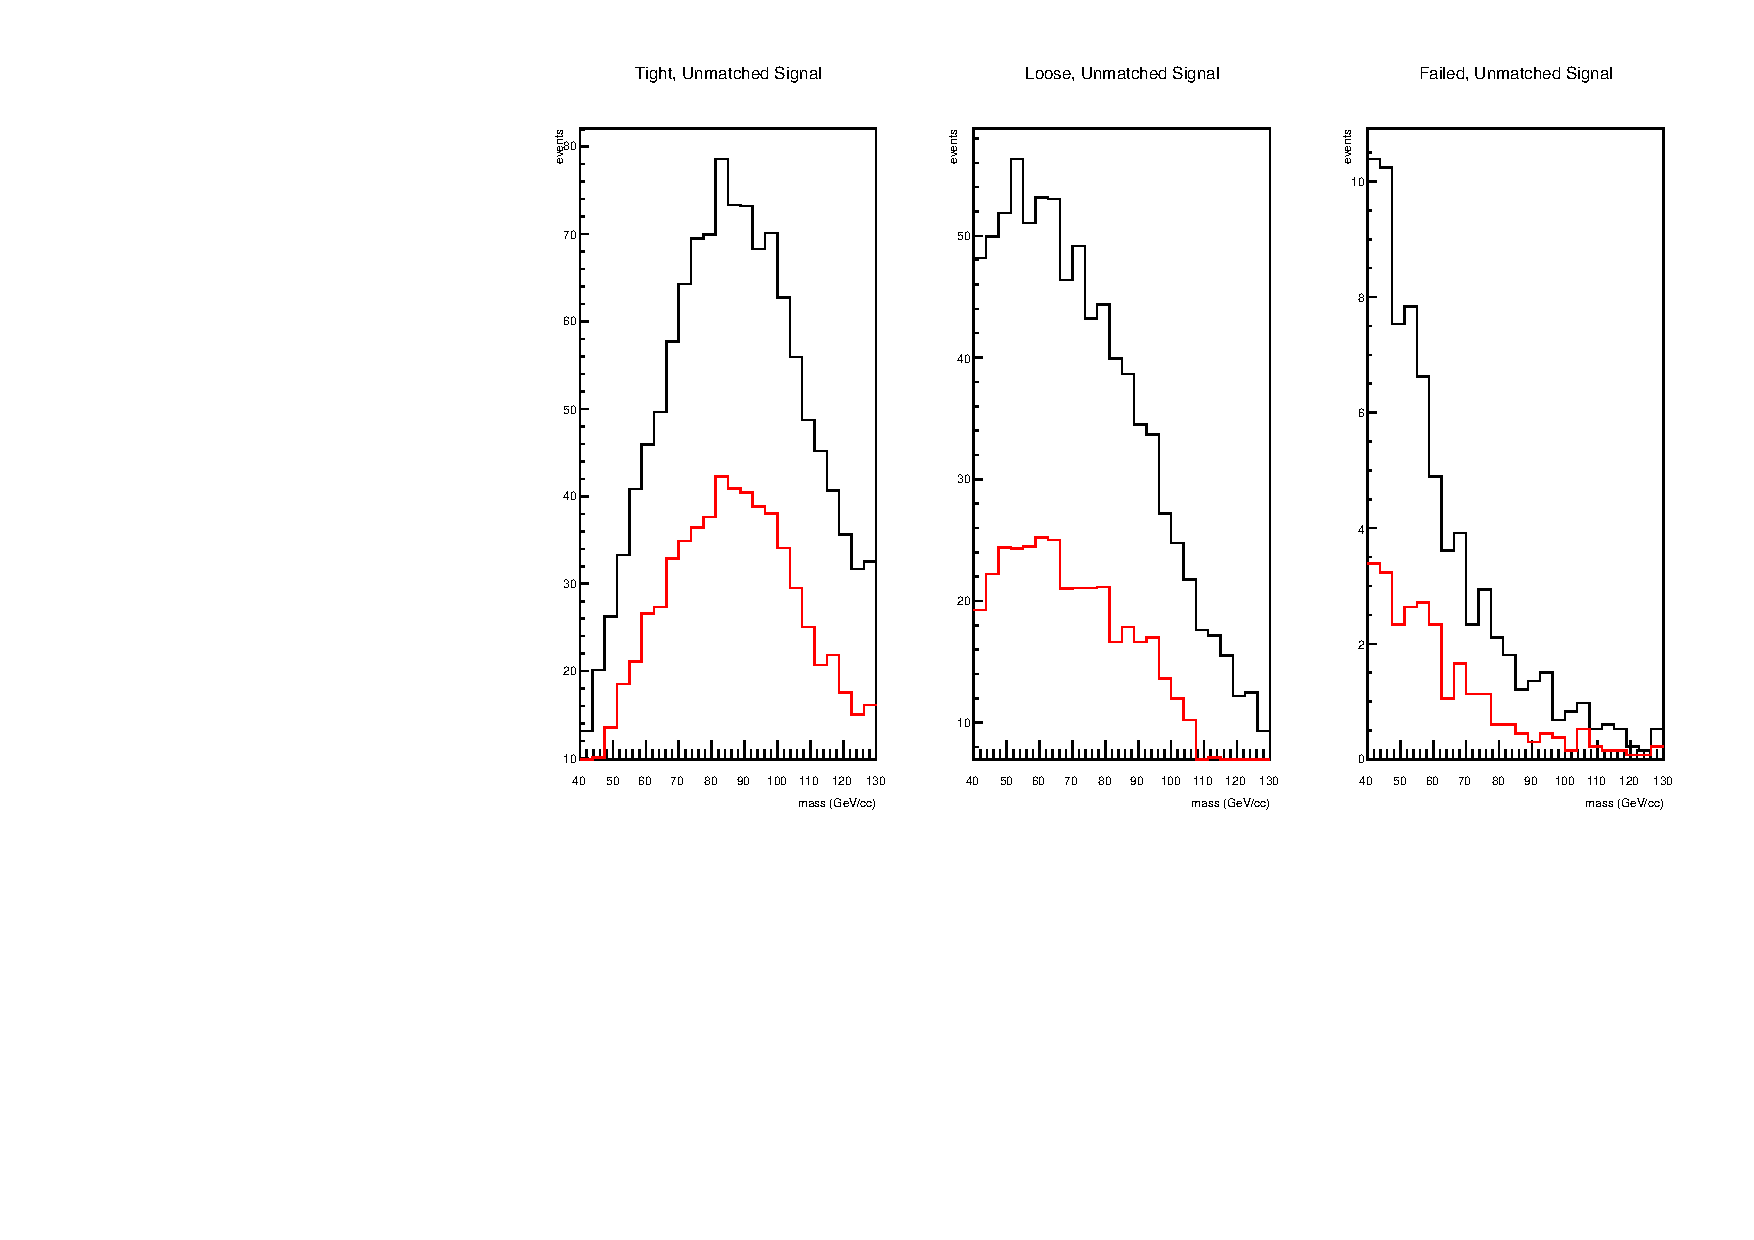
\includegraphics[width=0.77\textwidth]{EXO-12-024/figs/WtagSF/sigproofII.pdf}
    \caption{$W$-mass distributions in tight, loose and failed before(black) and after(red) the $\Delta R < 1.6$ cut.}\label{fig:drproof}
\end{figure}
\subsection{Distributions in MC}
In this section we show the fifteen different distributions which we will consider.
\subsubsection{Smoothing}
After the full selection, the backgrounds have low statistics in MC, and the resulting distributions yield fits with high errors. This affects all three of our backgrounds. xTo combat this, we loosen the selection and use the resulting distributions for fitting, normalizing them to the number of events passing the full-selection. The loose selection is as follows:
\begin{enumerate}
\item
No $b$-tag requirement.
\item
No isolation requirements on the muon (but we keep the $p_T$ cut).
\item
No hemisphere requirements on the $E^{miss}_T$.
\item
We do not apply the $\Delta R$ requirement on the $b$ and $W$ candidates.
\end{enumerate}
In figure \ref{fig:sbvalid} we can see the distribution of leptonic $t\overline{t}$ events in the full and loose selection. We've normalized the distributions, and can see that the looser selection doesn't cause a change in the shapes. The same process is applied to $W$+jets and single top backgrounds.
\begin{figure}[h!]
\centering
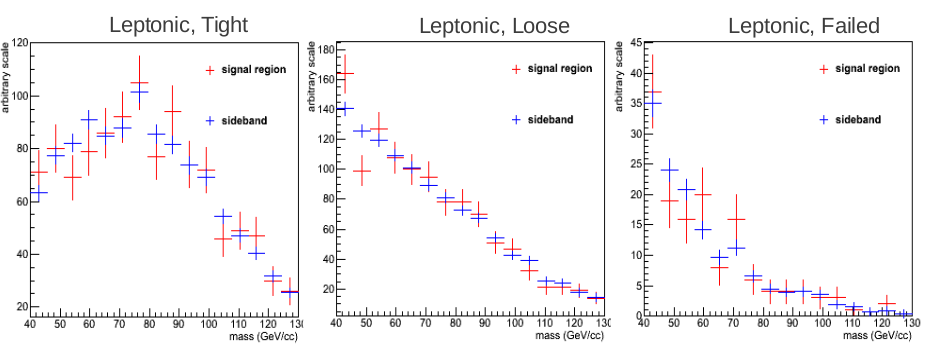
\includegraphics[scale=0.46]{EXO-12-024/figs/WtagSF/leptonicSB.png}
\caption{Agreement of the shapes in the loose and tight selection for leptonic $t\overline{t}$.}\label{fig:sbvalid}
\end{figure}
\subsubsection{Combined Distributions}
In figures \ref{fig:tightHIST}, \ref{fig:looseHIST}, and \ref{fig:failedHIST} the summed distributions of all components are shown. The smoothing of backgrounds has already been applied. All three histograms are normalized to our luminosity $\L = 19.7 fb^{-1}$.
\begin{figure}[h!]
\centering
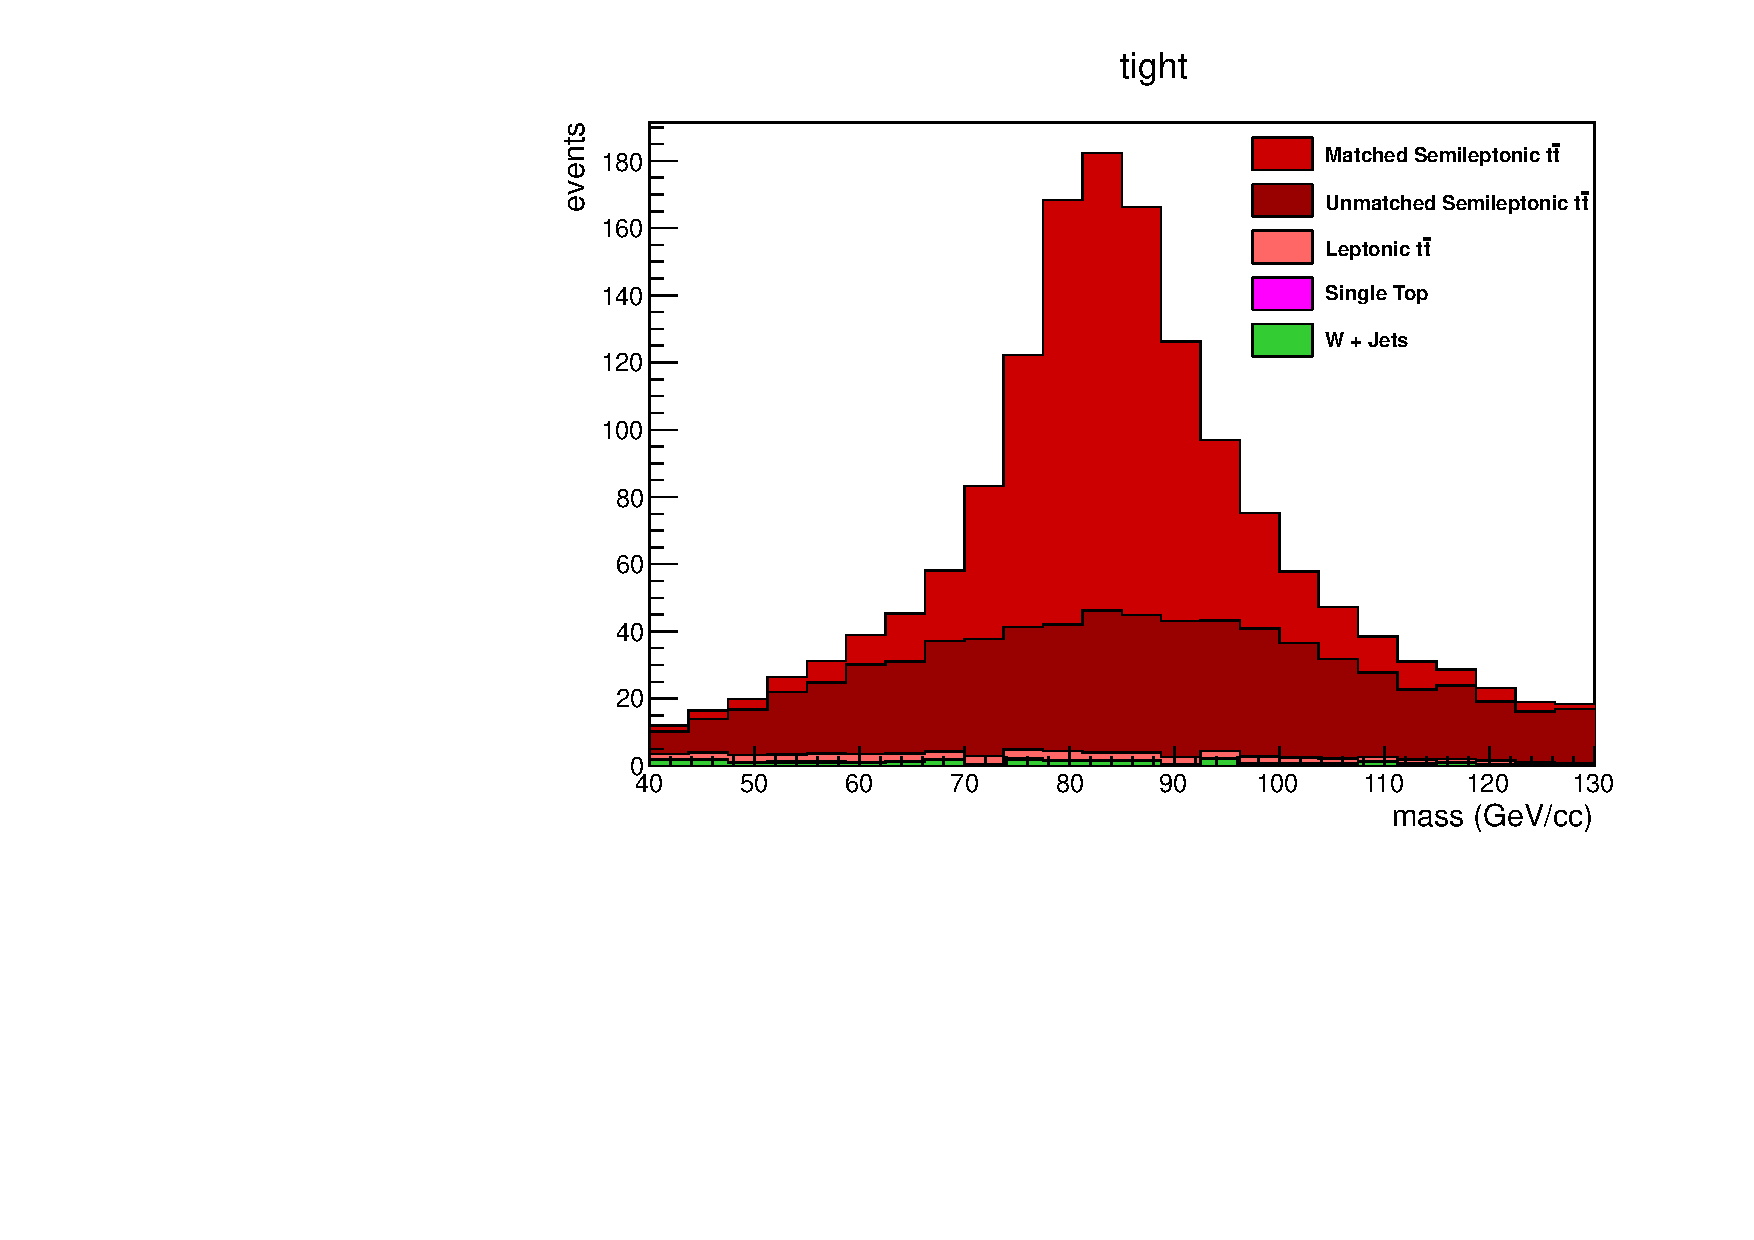
\includegraphics[scale=0.66]{EXO-12-024/figs/WtagSF/TOTAL_TIGHT.pdf}
\caption{Sum of all distributions passing the tight cut, normalized to our luminosity $\L = 19.7 fb^{-1}$.}\label{fig:tightHIST}
\end{figure}
\begin{figure}[h!]
\centering
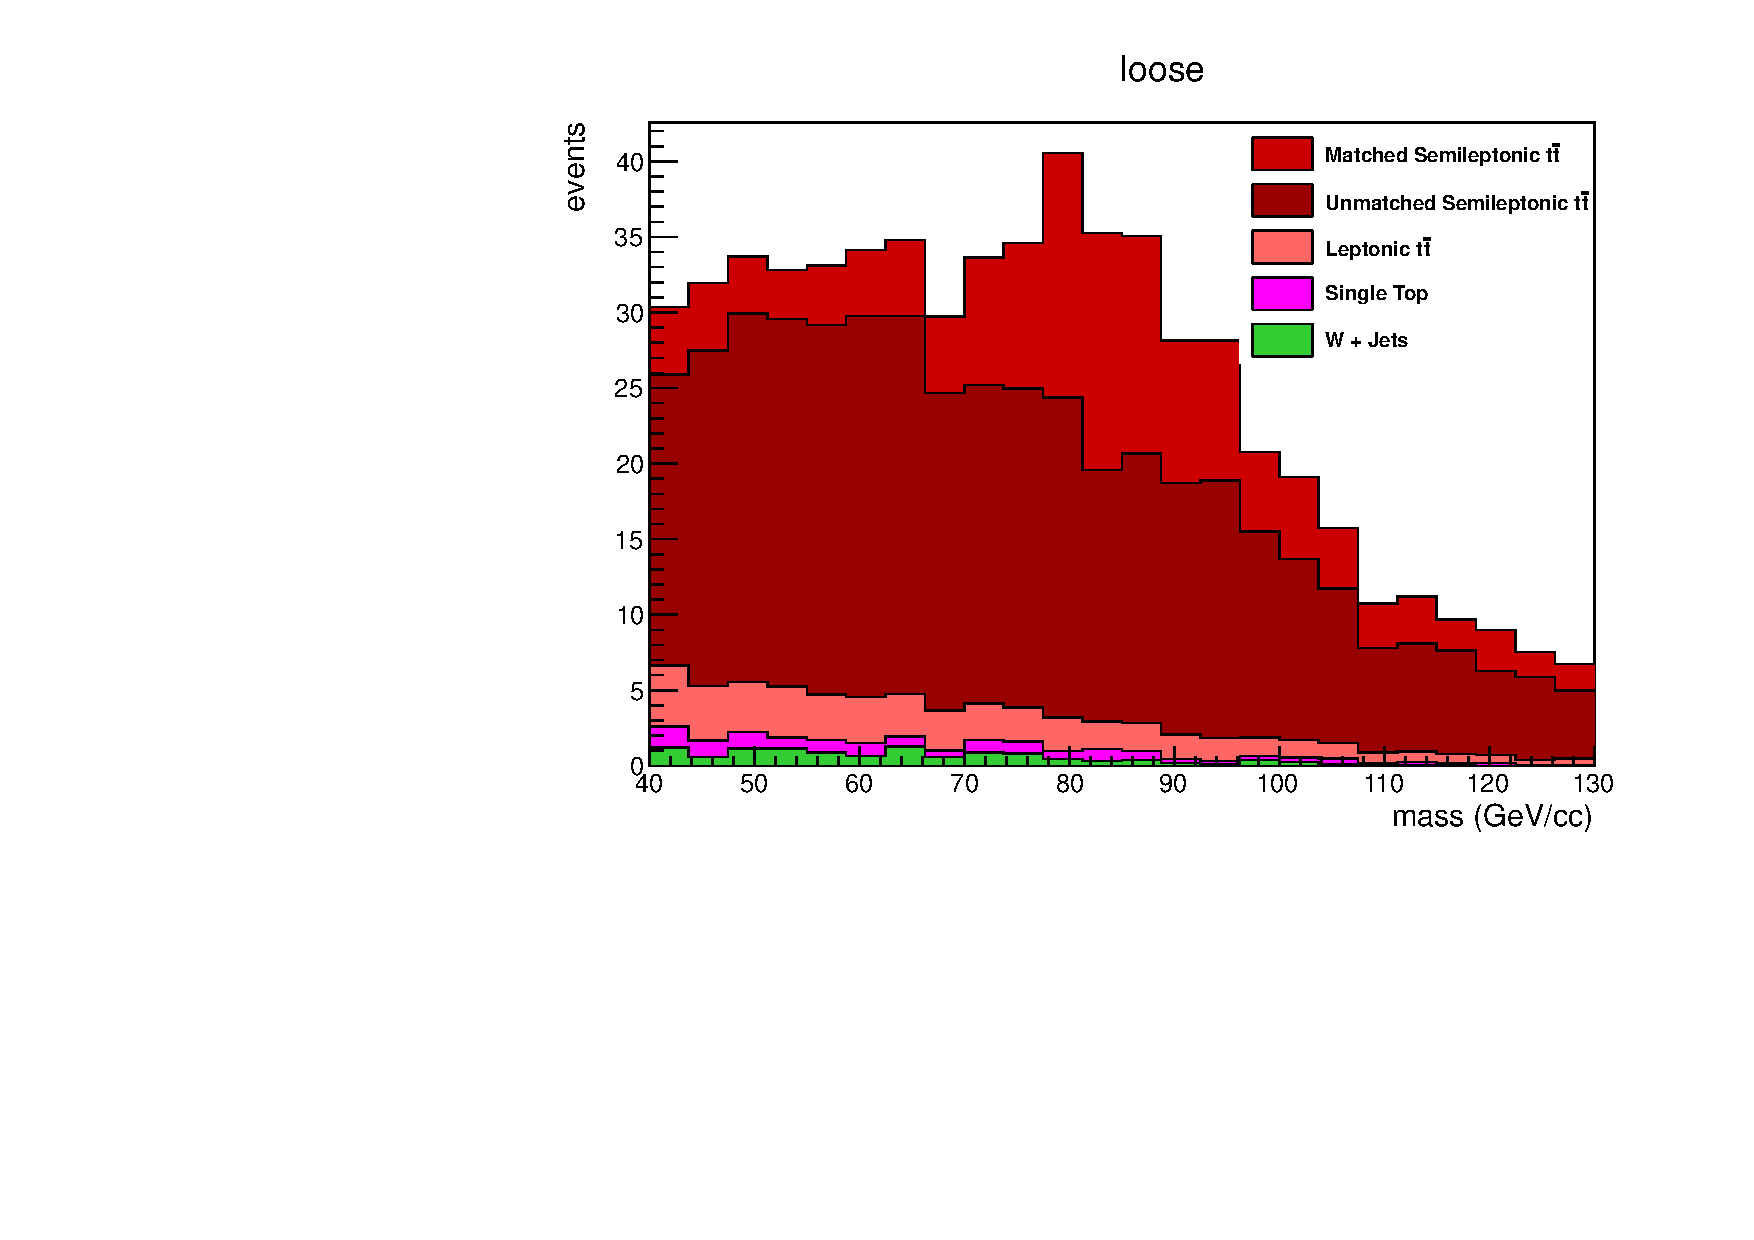
\includegraphics[scale=0.66]{EXO-12-024/figs/WtagSF/TOTAL_LOOSE.pdf}
\caption{Sum of all distributions passing the loose cut, normalized to our luminosity $\L = 19.7 fb^{-1}$.}\label{fig:looseHIST}
\end{figure}
\begin{figure}[h!]
\centering
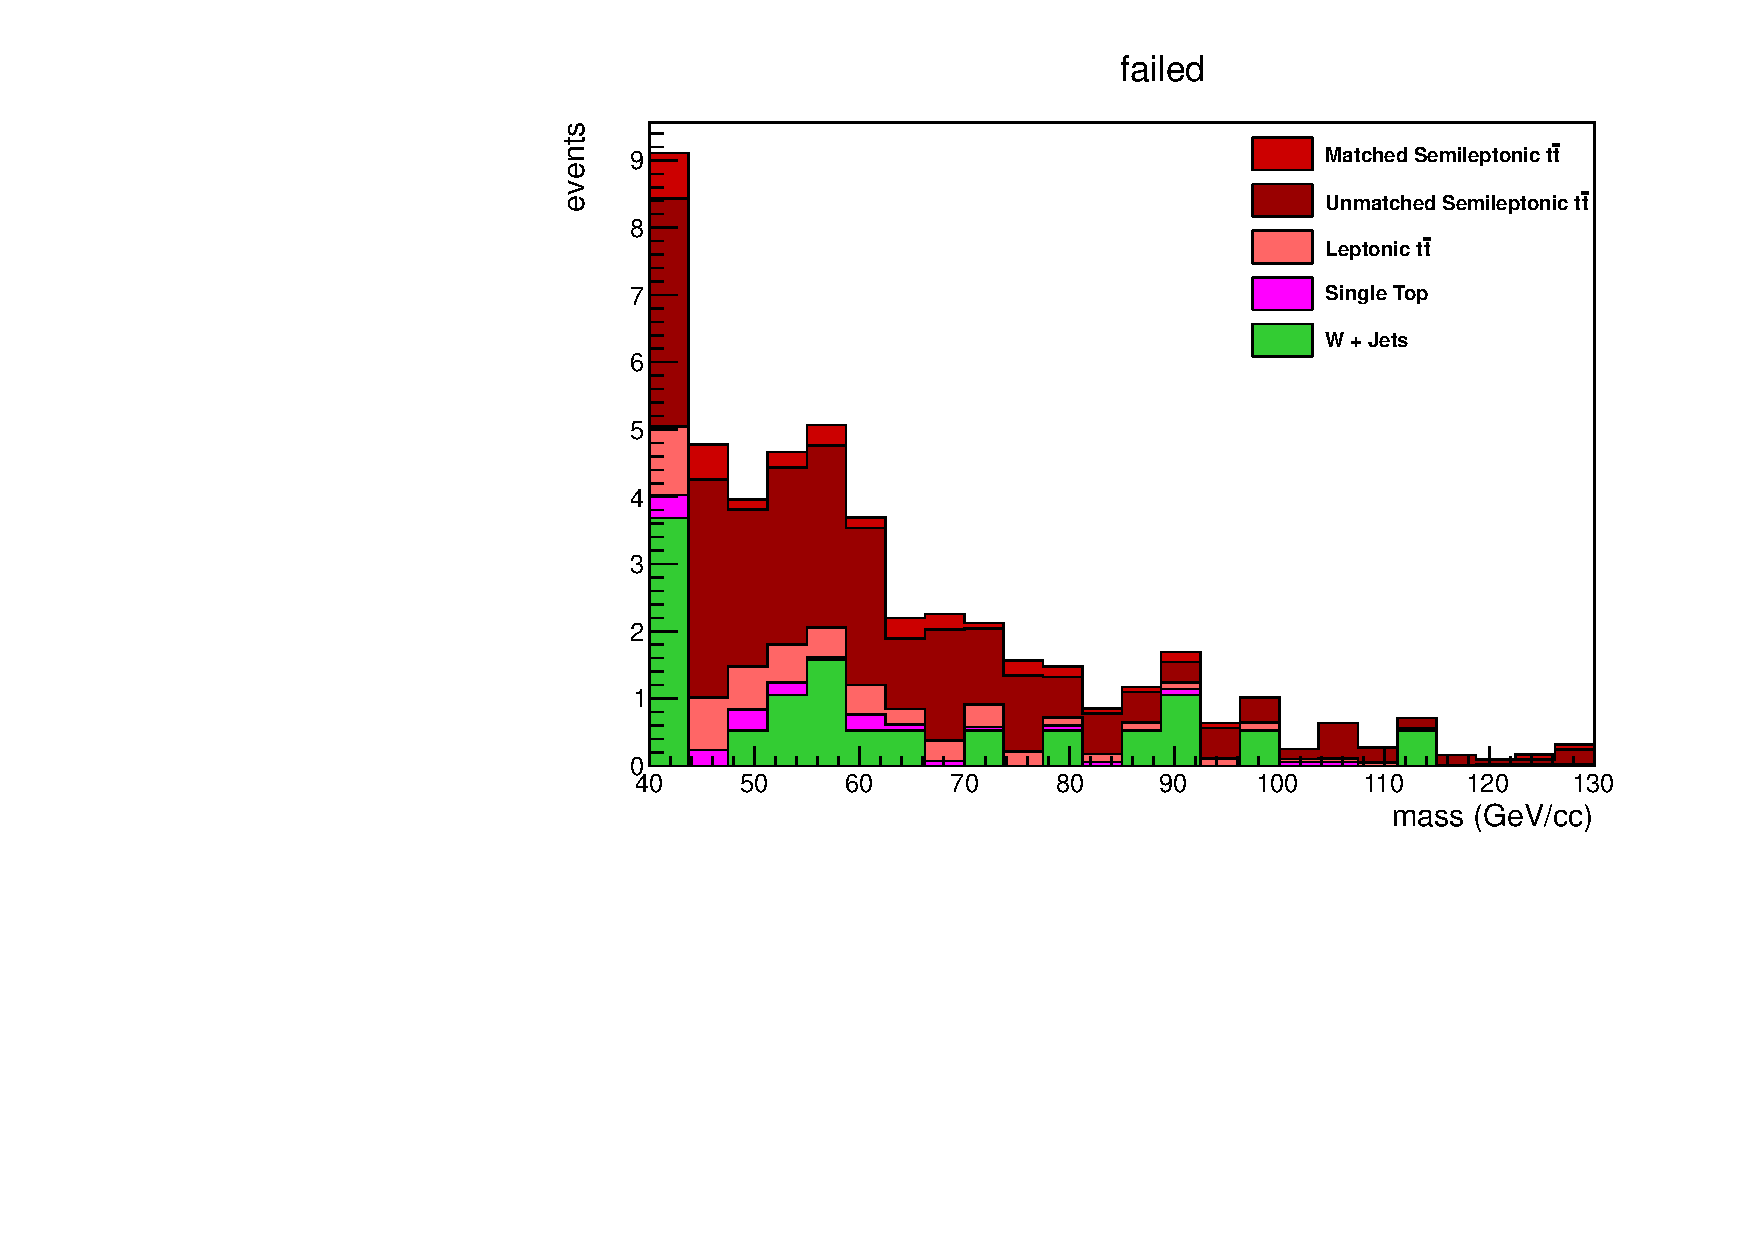
\includegraphics[scale=0.66]{EXO-12-024/figs/WtagSF/TOTAL_FAIL.pdf}
\caption{Sum of all distributions which failed both cuts, normalized to our luminosity $\L = 19.7 fb^{-1}$. }\label{fig:failedHIST}
\end{figure}
\subsection{Fitting Procedure}
We will attempt to isolate the true $W$s in data by fitting the constituent matched, unmatched and background components to the tight, loose and failed shapes in data.
\subsubsection{Background Shapes}
All backgrounds are fit with the same pdfs. The tight and loose shapes are fit to gaussians and the failed shapes are fit to decaying exponentials. There are thus $15$ parameters describing the shapes of the backgrounds. All of these parameters are held constant during the fit to data, but relative normalizations are allowed to vary during the fit. Table \ref{tab:mcval} lists the parameters describing the background, their values and the errors from fitting to MC. Plots of the resulting fits are shown in Figures \ref{fig:bkgI} - \ref{fig:bkgIII}
\begin{figure}[h!]
\centering
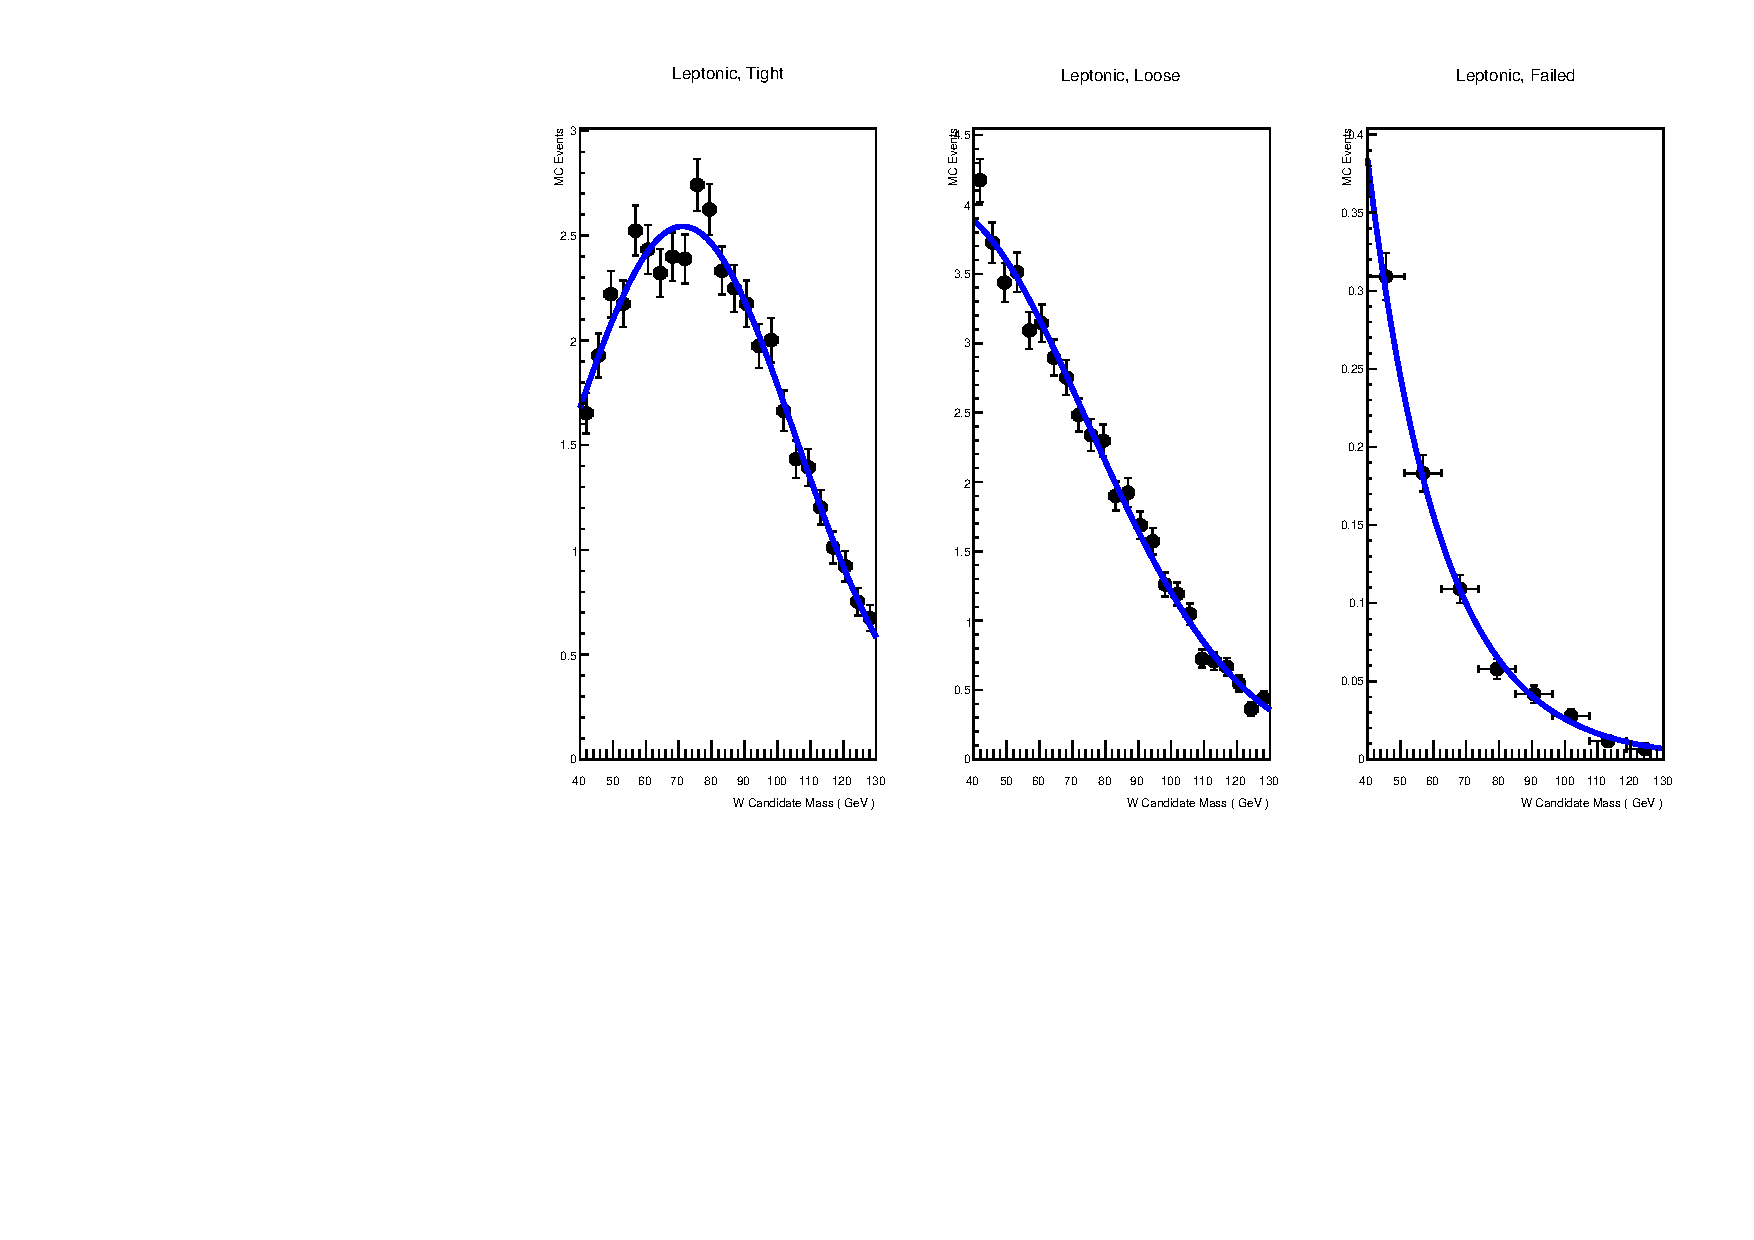
\includegraphics[scale=0.87]{EXO-12-024/figs/WtagSF/Leptonic_fits.pdf}
\caption{Fits to unmatched Leptonic distributions.}\label{fig:bkgI}
\end{figure}
\begin{figure}[h!]
\centering
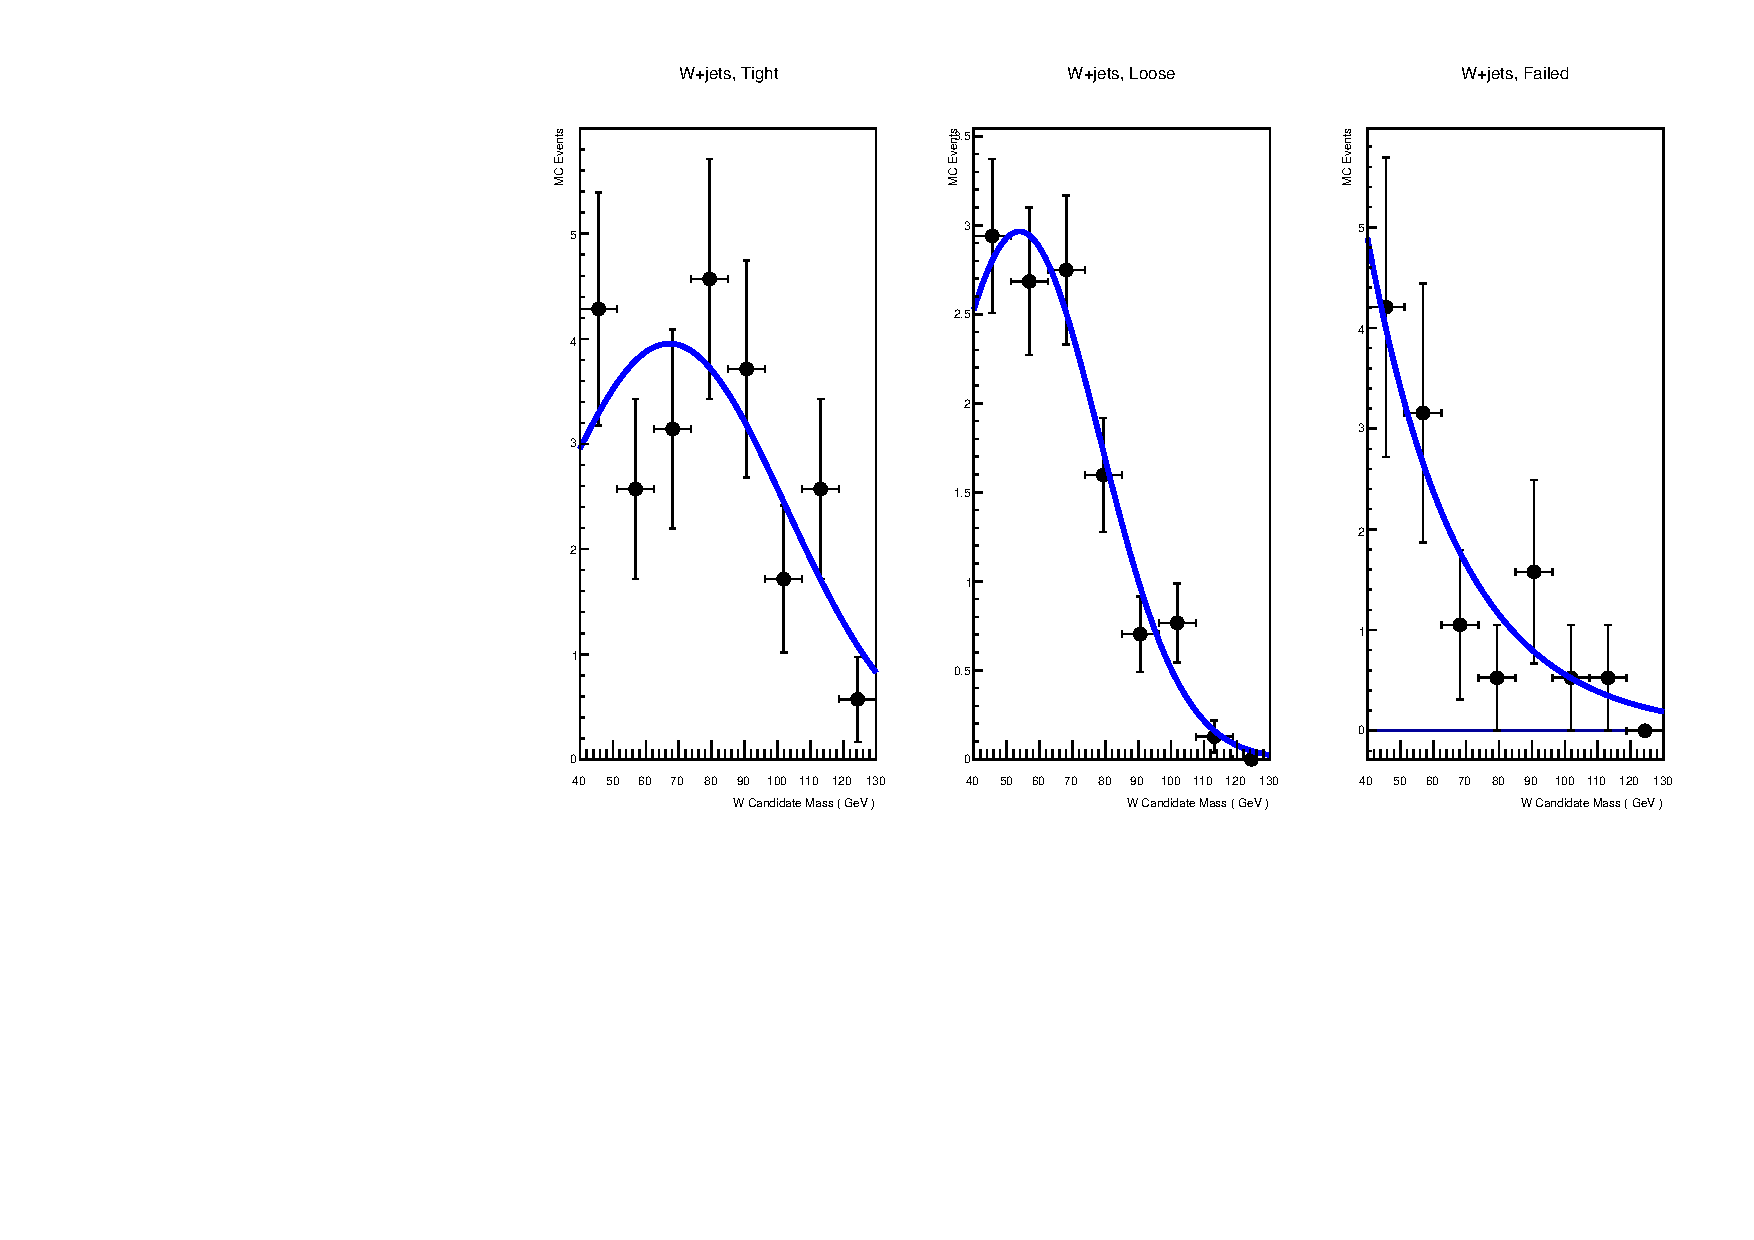
\includegraphics[scale=0.87]{EXO-12-024/figs/WtagSF/Wjets_fits.pdf}
\caption{Fits to unmatched W + jets distributions.}\label{fig:bkgII}
\end{figure}
\begin{figure}[h!]
\centering
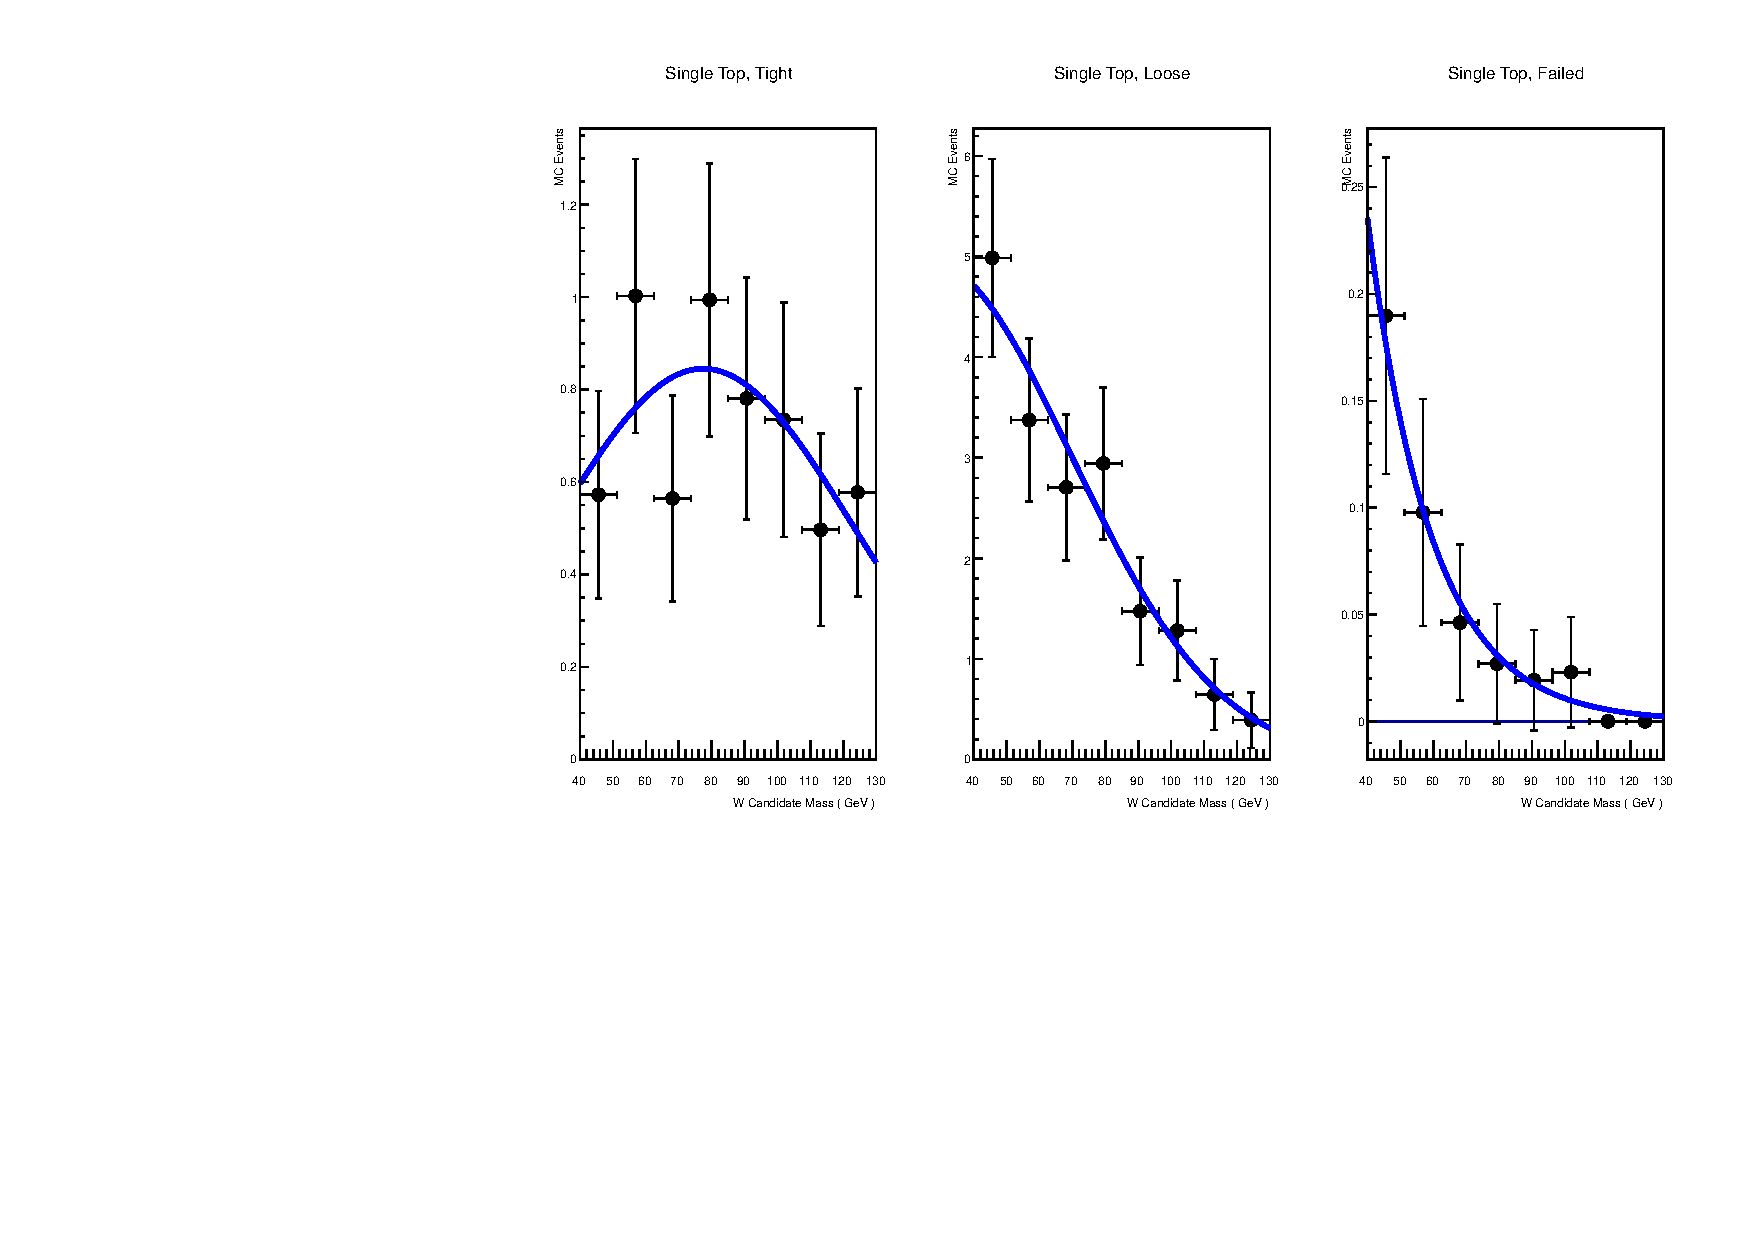
\includegraphics[scale=0.87]{EXO-12-024/figs/WtagSF/SingleTop_fits.pdf}
\caption{Fits to unmatched Single Top distributions.}\label{fig:bkgIII}
\end{figure}
\begin{table}
\centering
\begin{tabular}{l | c  c  c}
Background & variable & description & \\
\hline\hline
Leptonic $t\overline{t}$ & & & \\
& $\mu^l_T$ & Peak of Tight Gaussian & fixed in MC\\
\\
& $\sigma^l_T$ & Std Dev of Tight Gaussian & fixed in MC\\
\\
& $\mu^l_L$ & Peak of Loose Gaussian & fixed in MC\\
\\
& $\sigma^l_L$ & Std Dev of Loose Gaussian & fixed in MC\\
\\
& $\gamma^l_F$ & Decay coef of Failed Dist & fixed in MC\\
\\
\hline
W + jets & & & \\
& $\mu^w_T$ & Peak of Tight Gaussian & fixed in MC\\
\\
& $\sigma^w_T$ & Std Dev of Tight Gaussian & fixed in MC\\
\\
& $\mu^w_L$ & Peak of Loose Gaussian & fixed in MC\\
\\
& $\sigma^w_L$ & Std Dev of Loose Gaussian & fixed in MC\\
\\
& $\gamma^w_F$ & Decay coef of Failed Dist & fixed in MC\\
\\
\hline
Single Top & & & \\
& $\mu^t_T$ & Peak of Tight Gaussian & fixed in MC\\
\\
& $\sigma^t_T$ & Std Dev of Tight Gaussian & fixed in MC\\
\\
& $\mu^t_L$ & Peak of Loose Gaussian & fixed in MC\\
\\
& $\sigma^t_L$ & Std Dev of Loose Gaussian & fixed in MC\\
\\
& $\gamma^t_F$ & Decay coef of Failed Dist & fixed in MC\\
\\
\hline
\end{tabular}
\caption{Parameters used to describe the background distributions.} \label{tab:mcval}
\end{table}
\subsubsection{$t\overline{t}$ Shapes}
In the next sections we describe the shapes used to fit the $t\overline{t}$ distribution. Table \ref{tab:sigval} summarizes this discussion.
\subsubsection*{tight, unmatched}
For the tight, unmatched $t\overline{t}$ distribution, we use the sum of a gaussian distribution and a linear distribution. This yields four parameters, the mean and standard deviation of the gaussian, the slope of the line, and the relative normalization of the two shapes. When fit to data, the normalization is fixed to the value found by fitting to MC. All other parameters are allowed to float. The resulting fit is shown in Figure \ref{fig:unmatchedF}.
\subsubsection*{loose, unmatched}
The loose, unmatched $t\overline{t}$ distribution is fit to a gaussian. In the fit to data, the mean and standard deviation are both allowed to float. The resulting fit is shown in Figure \ref{fig:unmatchedF}.
\subsubsection*{failed, unmatched}
The failed, unmatched $t\overline{t}$ distribution is fit to an exponential. The coefficient is allowed to float. The resulting fit is shown in Figure \ref{fig:unmatchedF}.
\begin{figure}[h!]
\centering
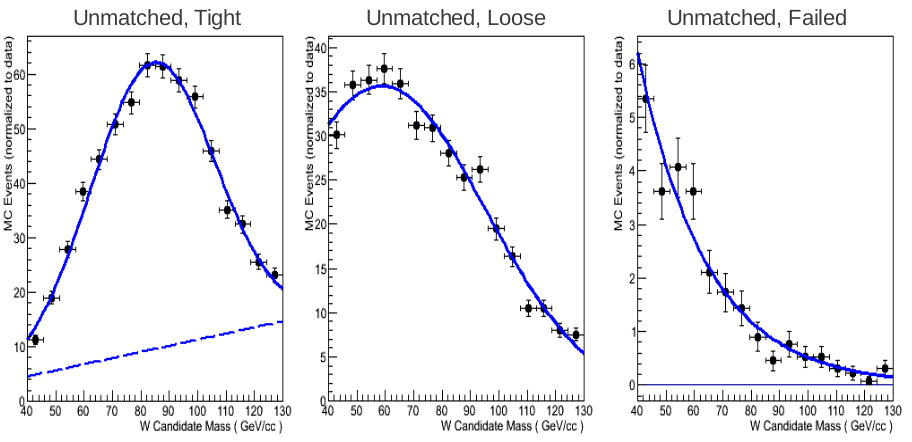
\includegraphics[scale=0.5]{EXO-12-024/figs/WtagSF/unmatched_fits.png}
\caption{Fits to unmatched $t\overline{t}$ distributions.}\label{fig:unmatchedF}
\end{figure}
\subsubsection*{tight and loose, matched}
The relative normalization of the tight and loose shapes are determined in part by the efficiency. This is not fit in MC. Instead, the shapes are determined on their own and the efficiency will only be taken into account when fitting to data. The tight shape and the loose shape however are related by the $W$-peak in the mass spectrum; the tight shape is just the peak, and the loose shape is the same peak with some added contribution from poorly merged $W$s which did nonetheless entered the loose selection (treated as an exponential decay. To account for this relation, the $W$-peak is fit for simultaneously in the tight and loose shapes. We fit the peak with the sum of two Gaussians. To simplify the eventual fit to data, the mean and sigma of the broader peak are expressed as multiples of the central peak's values. In our fit to data we will fix the dependence of the broader gaussian's parameters to that found in MC, allowing only the central peak's values to vary. The coefficient describing the exponential portion of the loose shape is also allowed to float. We will also fix the relative normalizations of the two gaussians and the relative normalization of the $W$-peak and exponential. All this information is summarized in Table \ref{tab:sigval} and the resulting fits are shown in Figure \ref{fig:matchedF}.

\subsubsection*{failed, matched}
The failed, matched shape is fit as an exponential, with all parameters allowed to float in the fit to data. See figure \ref{fig:unmatchedF}.
\begin{figure}[h!]
\centering
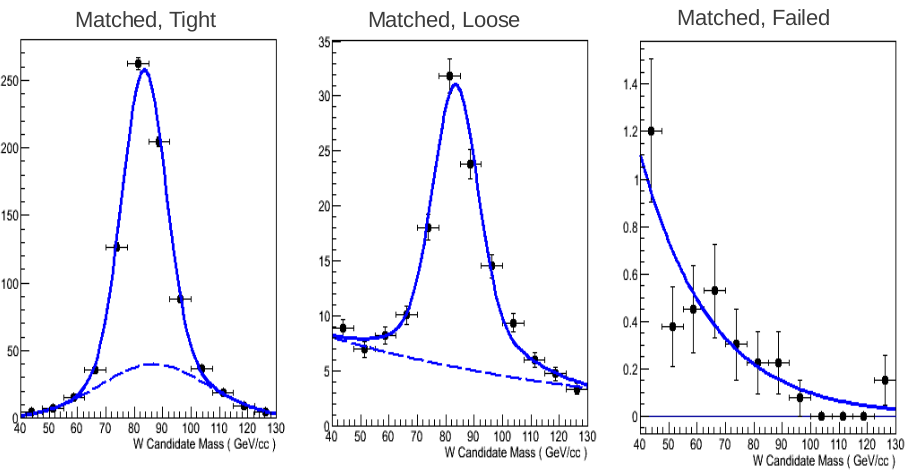
\includegraphics[scale=0.5]{EXO-12-024/figs/WtagSF/matched_fits.png}
\caption{Fits to matched $t\overline{t}$ distributions.}\label{fig:matchedF}
\end{figure}
We now have probability distribution functions for every component of the three mass distributions.
\begin{table}
\centering
\begin{tabular}{cccc}
Signal & variable & description & \\
\hline
Unmatched Tight &  $\mu^{ut}_T$ & Peak of Gaussian & fp\\
& $\sigma^{ut}_T$ & Std Dev of Gaussian & fp\\
& $m^{ut}_T$ & Slope of Linear Contribution & fp\\
& $f^{ut}_T$ & Relative normalization of & \textbf{fixed in MC}\\
& &  Linear and Gaussian Components &\\
\hline
Unmatched Loose&  $\mu^{ul}_L$ & Peak of Gaussian & fp\\
& $\sigma^{ul}_L$ & Std Dev of Gaussian & fp\\
\hline
Unmatched Failed & $\gamma^{uf}_F$ & Decay Coefficient & fp\\
\hline
Matched Tight/Loose & $\mu^{m}_P$ & Mean of $W$ Peak (Gaussian) & fp\\
& $\sigma^{m}_P$ & Std Dev of $W$ Peak & fp\\
& $\mu^{m}_S$ & Peak of Secondary Gaussian & \textbf{fixed w.r.t $\mu^{m}_P$}\\
& $\sigma^{m}_S$ & Std Dev of Secondary Gaussian & \textbf{fixed w.r.t $\mu^{m}_P$}\\
& $f^{m}_P$ & Relative normalization of & \textbf{fixed in MC}\\
& &  above two Gaussians &\\
& $\gamma^{m}_L$ & Decay Coefficient of unmerged $W$s & fp\\
& $f^{ut}_T$ & Relative normalization of & \textbf{fixed in MC}\\
& &  Merged and Unmerged events in Loose &\\
\hline
Matched Failed & & & \\
\hline
\end{tabular}
\caption{Parameters used to describe the signal distributions. fp is shot for 
floating parameter.} 
\label{tab:sigval}
\end{table}

\subsection{Efficiency Calculation}
We will simultaneously fit the shapes found in MC to the three mass-distributions in data. We can calculate the efficiency in data by making it a parameter in the fit. 
We define the following internal efficiencies: 
\begin{equation}
\epsilon^T_{matched},\epsilon^{L\star}_{matched},\epsilon^T_{unmatched}, \epsilon^{L\star}_{unmatched}, \epsilon^T_{bkg}, \epsilon^{L\star}_{bkg}
\end{equation}
Note that $\epsilon^{L\star}$ is not the efficiency of the loose cut, but rather, the efficiency for sorting events which have failed the tight cut into either loose or failed events. Defining this efficiency makes the mathematics easier to handle in the RooFit coding environment. 
The efficiencies and normalizations are related by the following equations, which contain all the necessary constraints on the fit. Bold values are fixed values taken form integrating the distributions in data. All other values are allowed to float during the fit.
We first set up equations relating the number of events expected in the backgrounds and unmatched shapes:
\begin{eqnarray}
BT & = & TB\times \epsilon^T_{bkg}\\
BL & = & TB\times (1 - \epsilon^T_{bkg}) \times \epsilon^{L\star}_{bkg}\\
BF & = & TB - (BT + BL)) \\
UT & = & TU\times \epsilon^T_{unmatched}\\
UL & = & TU\times (1 - \epsilon^T_{unmatched}) \times \epsilon^{L\star}_{unmatched}\\
UF & = & TU - (UT + UL) \\
\end{eqnarray}
Where: $TU$ and $TB$ are the total unmatched and background events respectively. To find the total matched events (TM), we use:
\begin{equation}
TM = (\textbf{TT}- (UT + BT)) + (\textbf{TL}- (UL + BL)) + (\textbf{TF}- (UF + BF))
\end{equation}
From which we can find the efficiencies by requiring:
\begin{eqnarray}
MT & = & TM\times \epsilon^T_{matched}\\
ML & = & TM\times (1 - \epsilon^T_{matched}) \times \epsilon^{L\star}_{matched}\\
MF & = & TM - (MT + ML)) \\
\end{eqnarray}
\clearpage
